\apendice{Manual de especificación de diseño}

\section{Planos}

Para este proyecto, se incluye un diagrama detallado del prototipo de dispositivo de monitoreo. Este plano muestra todas las conexiones eléctricas y la configuración del hardware. Se presenta el esquema que ilustra cómo están conectados los componentes principales como el sensor AD8232, Arduino y otros componentes.

\begin{figure}[h]
\centering
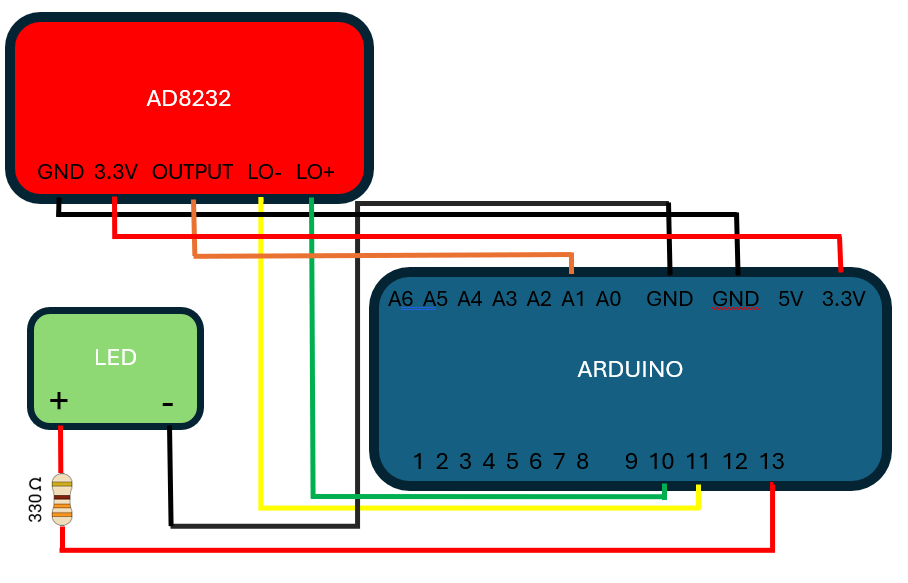
\includegraphics[width=\textwidth]{img/esquema.png}
\caption{Esquema prototipo de Arduino}
\label{fig:esquema}
\end{figure}

Como se muestra en la Figura \ref{fig:esquema}, este esquema ayuda a entender la disposición física de los componentes y es esencial para la replicación o modificación del prototipo. Detalla a que pin del microcontrolador Arduino esta conectado cada componente usado en el proyecto.

Además, se presenta el resultado final del hardware en el siguiente esquema:

\begin{figure}[h]
\centering
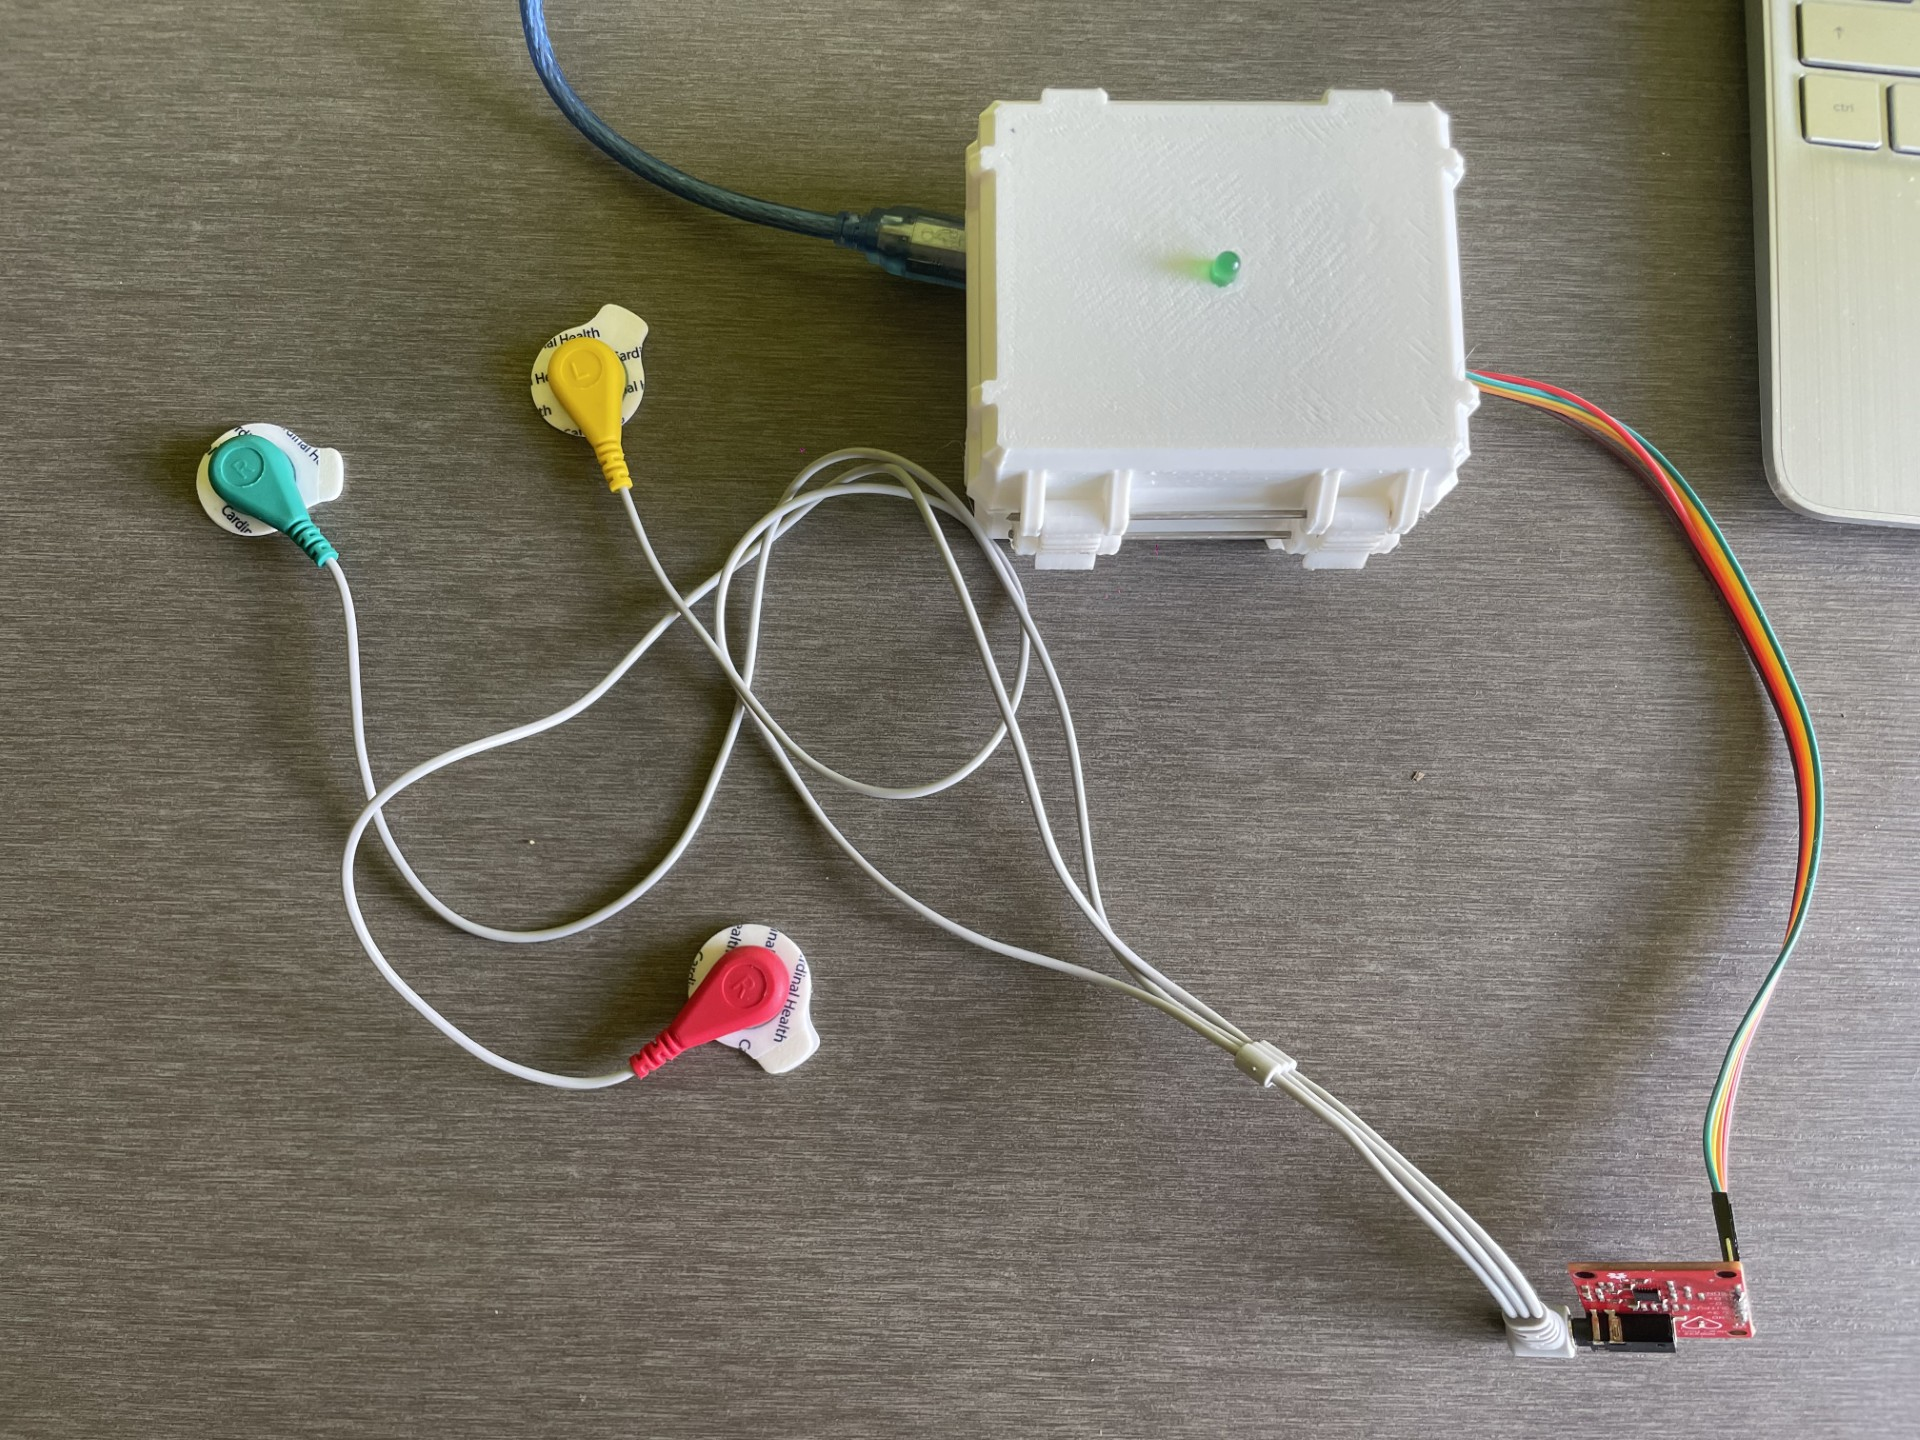
\includegraphics[width=\textwidth]{img/proyecto.jpg}
\caption{Montaje final del hardware}
\label{fig:final}
\end{figure}

La Figura \ref{fig:final} es el diseño final del prototipo, mostrando cómo se integran todos los componentes en un ensamble compacto y funcional. Este diseño final es el resultado de diferente pruebas y ajustes, para que el dispositivo sea ergonómico y cómodo para el usuario.

\section{Diseño arquitectónico}

El diseño arquitectónico del proyecto combina tanto software como hardware, representado mediante diagramas de flujo claros y fáciles de entender. Estos diagramas ayudan a visualizar cómo funciona el sistema desde la carga inicial del software en el dispositivo hasta el análisis de los datos.

\subsection{Diagrama de Arduino}

El primer diagrama, Figura \ref{fig:diagrama1}, muestra los pasos para preparar el Arduino. Este proceso incluye cómo se carga el software necesario para que el Arduino pueda empezar a trabajar con los sensores y recoger datos.

\begin{figure}[h]
\centering
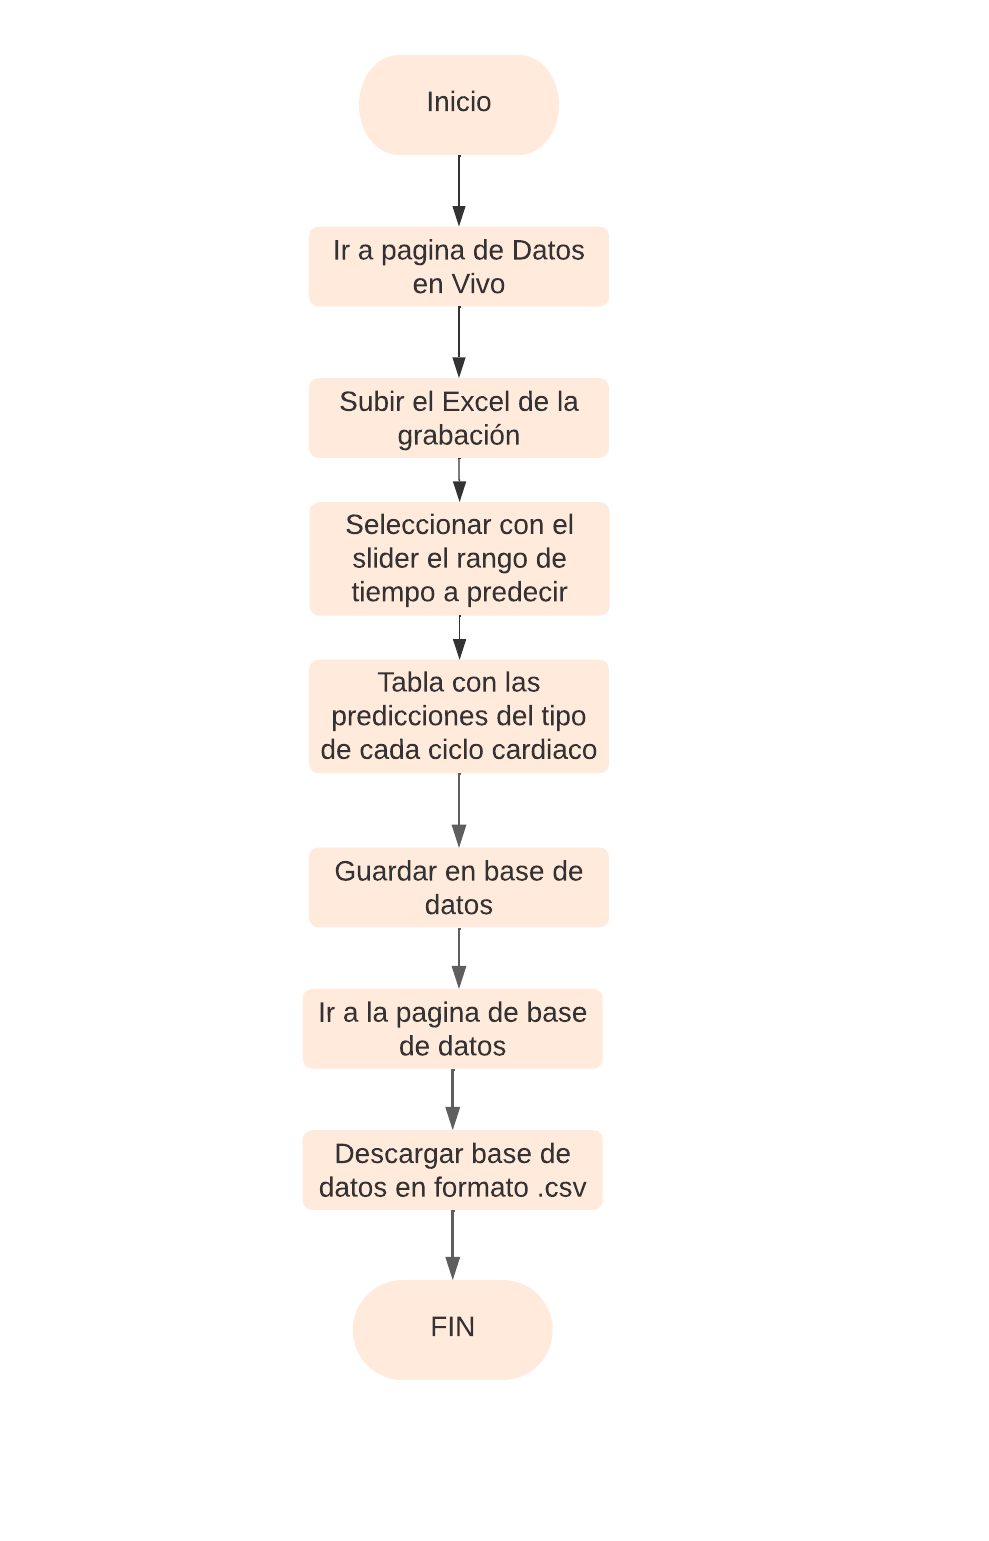
\includegraphics[width=\textwidth]{img/Diagramas/Diagrama_analisis.png}
\caption{Diagrama de flujo para configurar Arduino}
\label{fig:diagrama1}
\end{figure}

\subsection{Diagrama de datos en vivo}

El segundo diagrama, Figura \ref{fig:diagrama2}, explica cómo se recogen y se almacenan los datos del corazón en tiempo real. Este diagrama muestra desde el inicio de la grabación de los datos hasta su almacenamiento, asegurando que los datos se guarden correctamente para su uso posterior.

\begin{figure}[h]
\centering
\includegraphics[width=\textwidth]{img/Diagramas/diagrama_datosvivo.png}
\caption{Diagrama de flujo del proceso de grabación de datos en tiempo real}
\label{fig:diagrama2}
\end{figure}

\subsection{Diagrama de análisis}

El tercer diagrama, Figura \ref{fig:diagrama3}, detalla cómo se hace para analizar los datos del corazón que se han grabado. Este proceso abarca desde cargar los datos ya recogidos hasta analizarlos y guardarlos en la base de datos junto a la fecha y hora para despues descargarlo en formato .csv.

\begin{figure}[h]
\centering
\includegraphics[width=\textwidth]{img/Diagramas/diagrama_analisis.png}
\caption{Diagrama de flujo del análisis de datos del corazón}
\label{fig:diagrama3}
\end{figure}

Estos diagramas ofrecen una forma sencilla y organizada de entender las principales funciones del proyecto, haciendo más accesible para cualquier persona la información técnica y facilitando el trabajo de futuras mejoras o expansiones del sistema.


